\section{Definició de conceptes}
\subsubsection{Anàlisi d'un tiquet}
Un tiquet d'incidències és un informe de qualsevol problema o dubte que hagi pogut sorgir, normalment, dins d'una empresa. Aquests tiquets serveixen per comunicar del problema mencionat al tiquet i s'espera obtenir una contestació detallant quins són els passos a seguir per solucionar el problema o una resposta resolent el dubte. Per aquest projecte, s'utilitza OTRS, una eina de gestió i emmagatzematge de tiquets. A continuació, es mostra un tiquet d'exemple d'ORTS i s'explica en deteniment les seves parts.
%(usuaris afectats, accions mitigació, accions control, url mail incident, from mail incident, recipient mail incident, subject mail incident)

En el tiquet es pot veure els següents camps:
\begin{enumerate}
    \item \textbf{Logo Znuny:} Tot i que a l'agència s'utilitza OTRS, aquest tiquet d'exemple, i les proves que s'han dut a terme han sigut realitzades amb Znuny. Znuny és la continuació d'OTRS, ja que a partir en un cert punt, la versió gratuita d'OTRS (OTRS Community Edition) va deixar de rebre actualitzacions de manteniment. A efectes pràctics, Znuny és compatible amb les mateixes llibreries que OTRS i es comporta de manera idèntica. S'utilitzarà per a totes les proves locals que requereixin el servei d'un gestor de tiquets.
    \item \textbf{Nombre del tiquet:} Nombre identificador únic del tiquet. És l'identificador principal per obtenir el tiquet de la base de dades.
    \item \textbf{Capçalera:} Els tiquets tenen un assumpte, remitent, destinatari i informació sobre la data d'enviament; igual que un correu electrònic. En aquest cas, està dividida en diversos llocs del tiquet.
    \item \textbf{Informació del tiquet (metadata):} Hi ha informació inclosa en el tiquet que permet establir alguns camps rellevants relatius a les condicions actuals del tiquet, tals com: l'estat del tiquet, la seva prioritat, a quina cua pertany, quant de temps fa que s'ha creat, etc.
    \item \textbf{Informació del client:} Conté informació sobre l'empresa que ha patit l'incident, així com l'usuari de l'empresa que ha escrit el tiquet.
    \item \textbf{Nombre de l'article:} Un tiquet es divideix en diferents articles. Cada article representa un missatge o correu que una de les parts ha fet. En aquest exemple hi ha dos articles: El primer (\ref{fig:tiquet-exemple-2}) informant del problema i el segon (\ref{fig:tiquet-exemple-1}) explicant les mesures preses a causa de l'incident. És important tenir en compte que, tal com es veu a la Figura \ref{fig:tiquet-exemple-1}, el text de tots els anteriors tiquets es reescriu sota d'aquest.
\end{enumerate}

\begin{figure}[H]
    \centering
    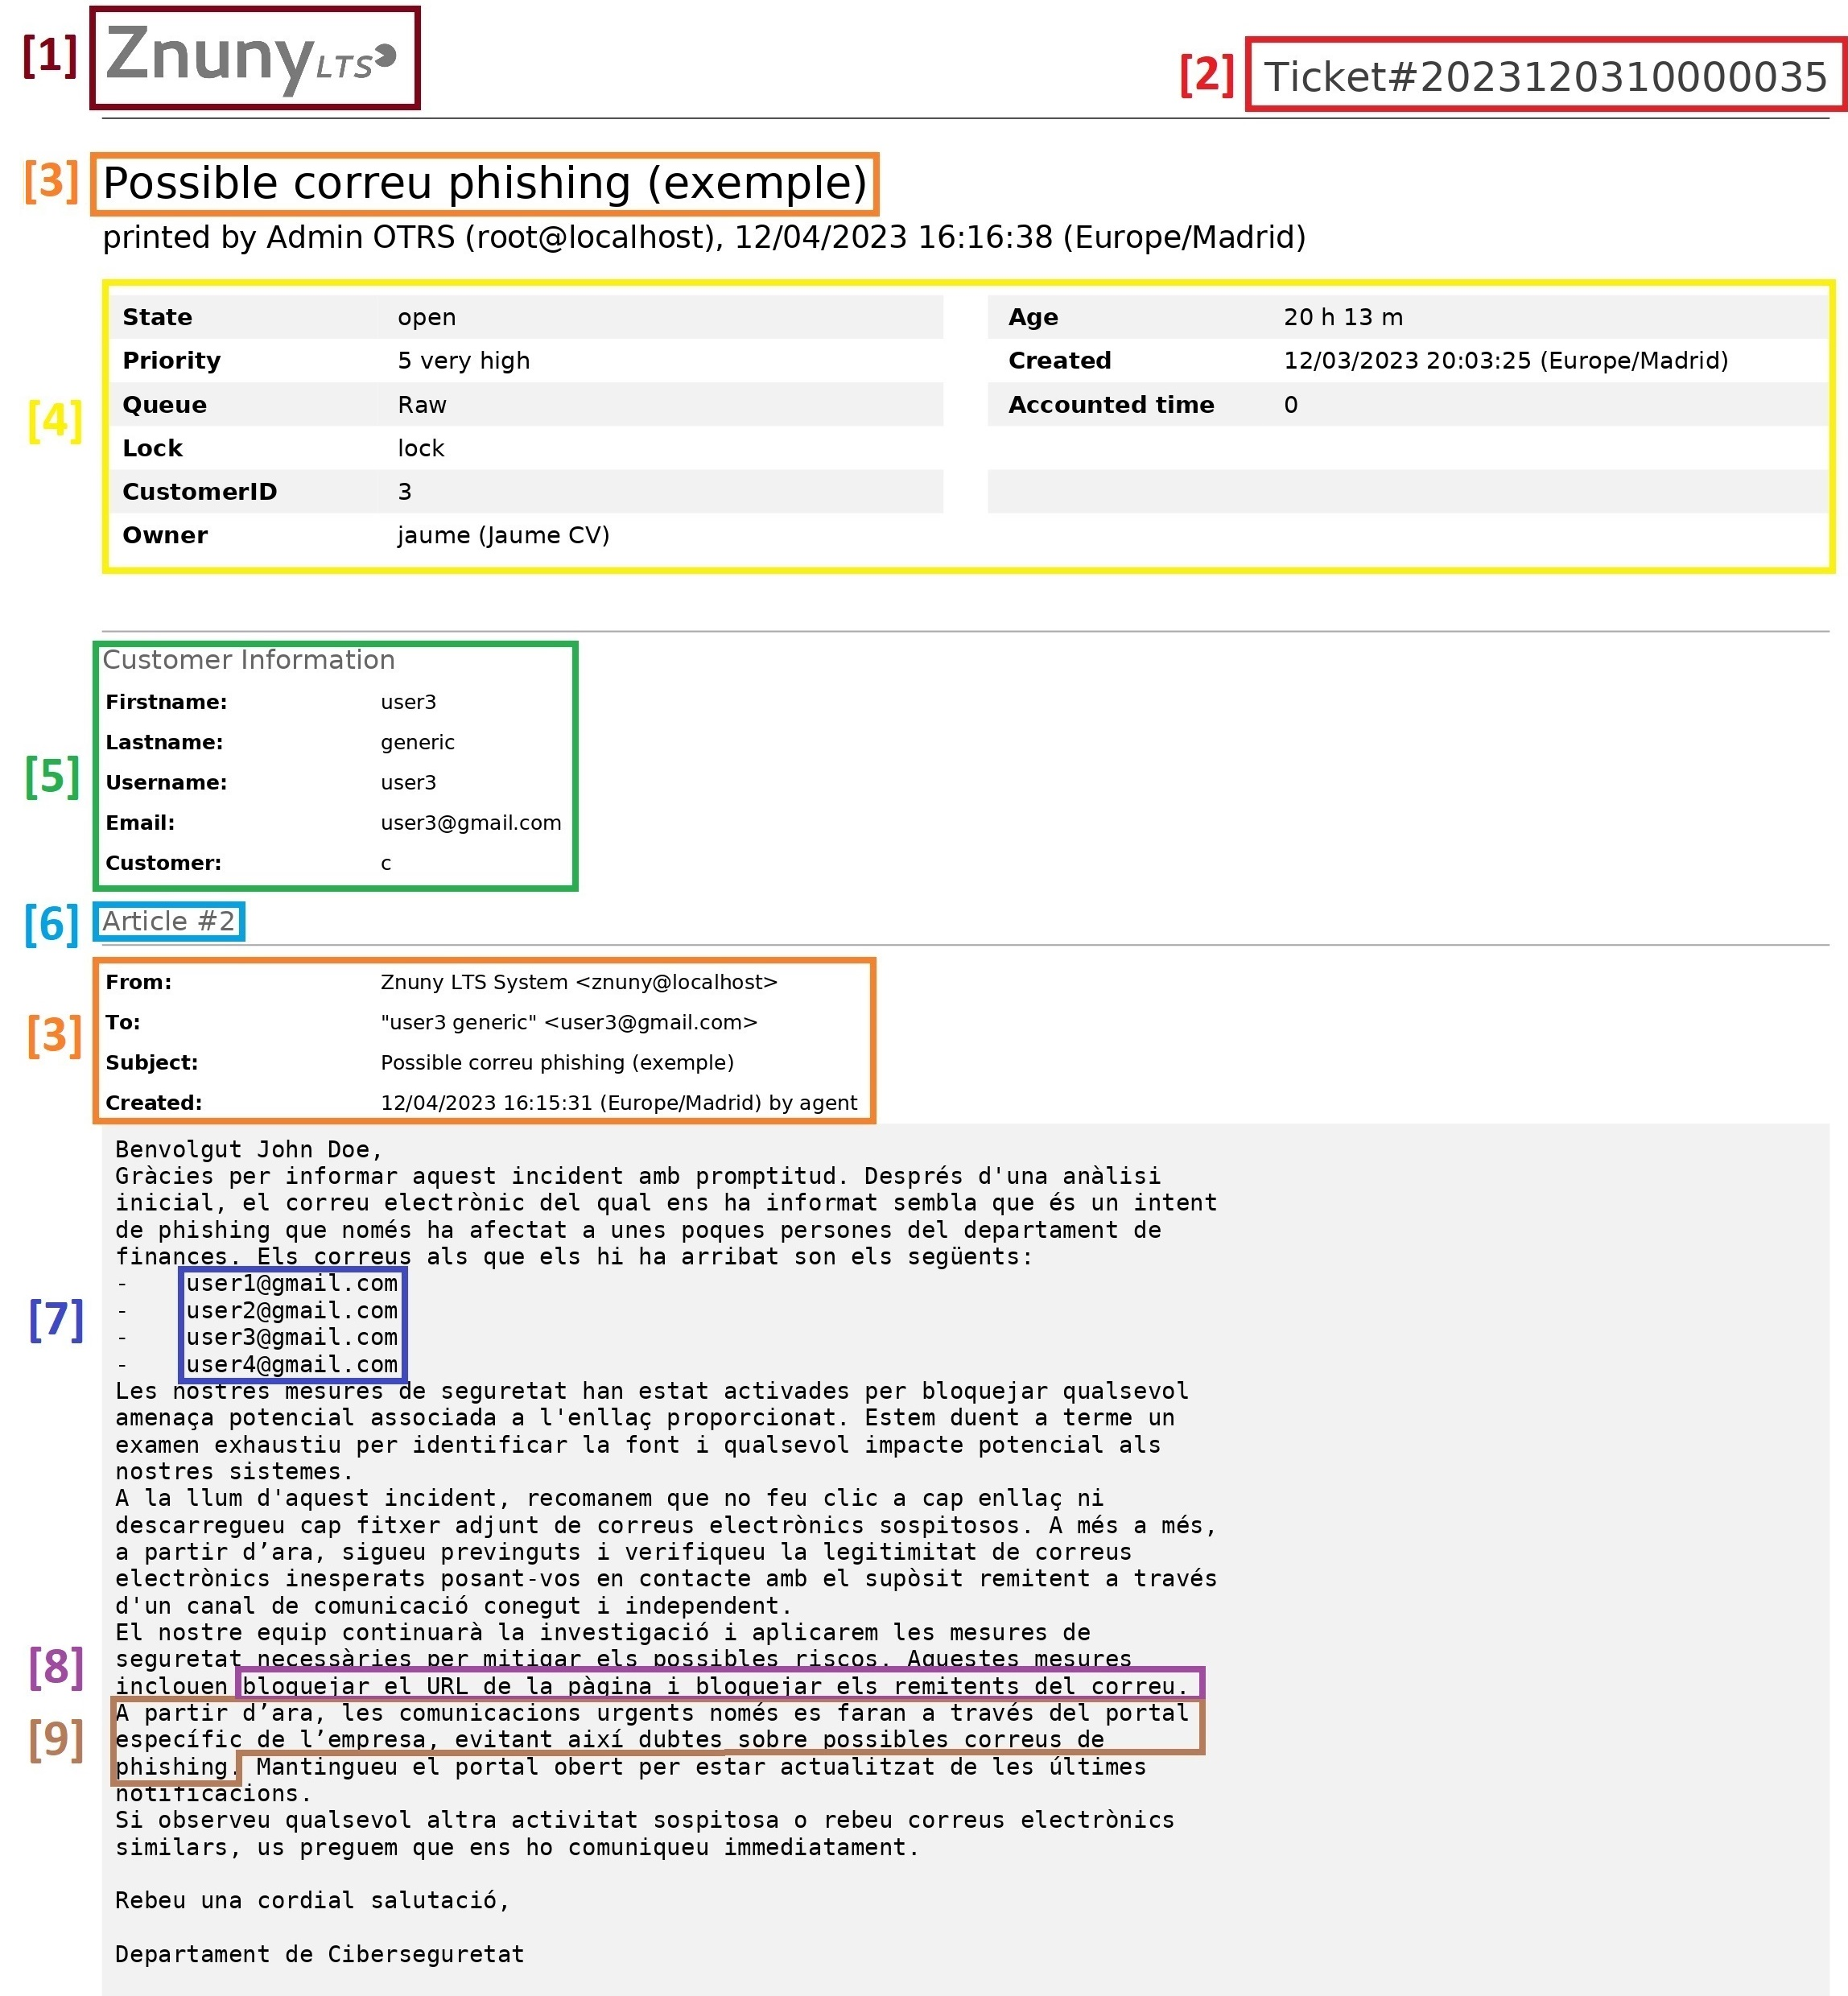
\includegraphics[width=\textwidth]{meitat-1.png}
    \caption{Primera meitat del tiquet d'exemple d'ORTS amb totes les parts indicades. \\ \textit{(Creació pròpia)}}
    \label{fig:tiquet-exemple-1}
\end{figure}


\begin{figure}[H]
    \centering
    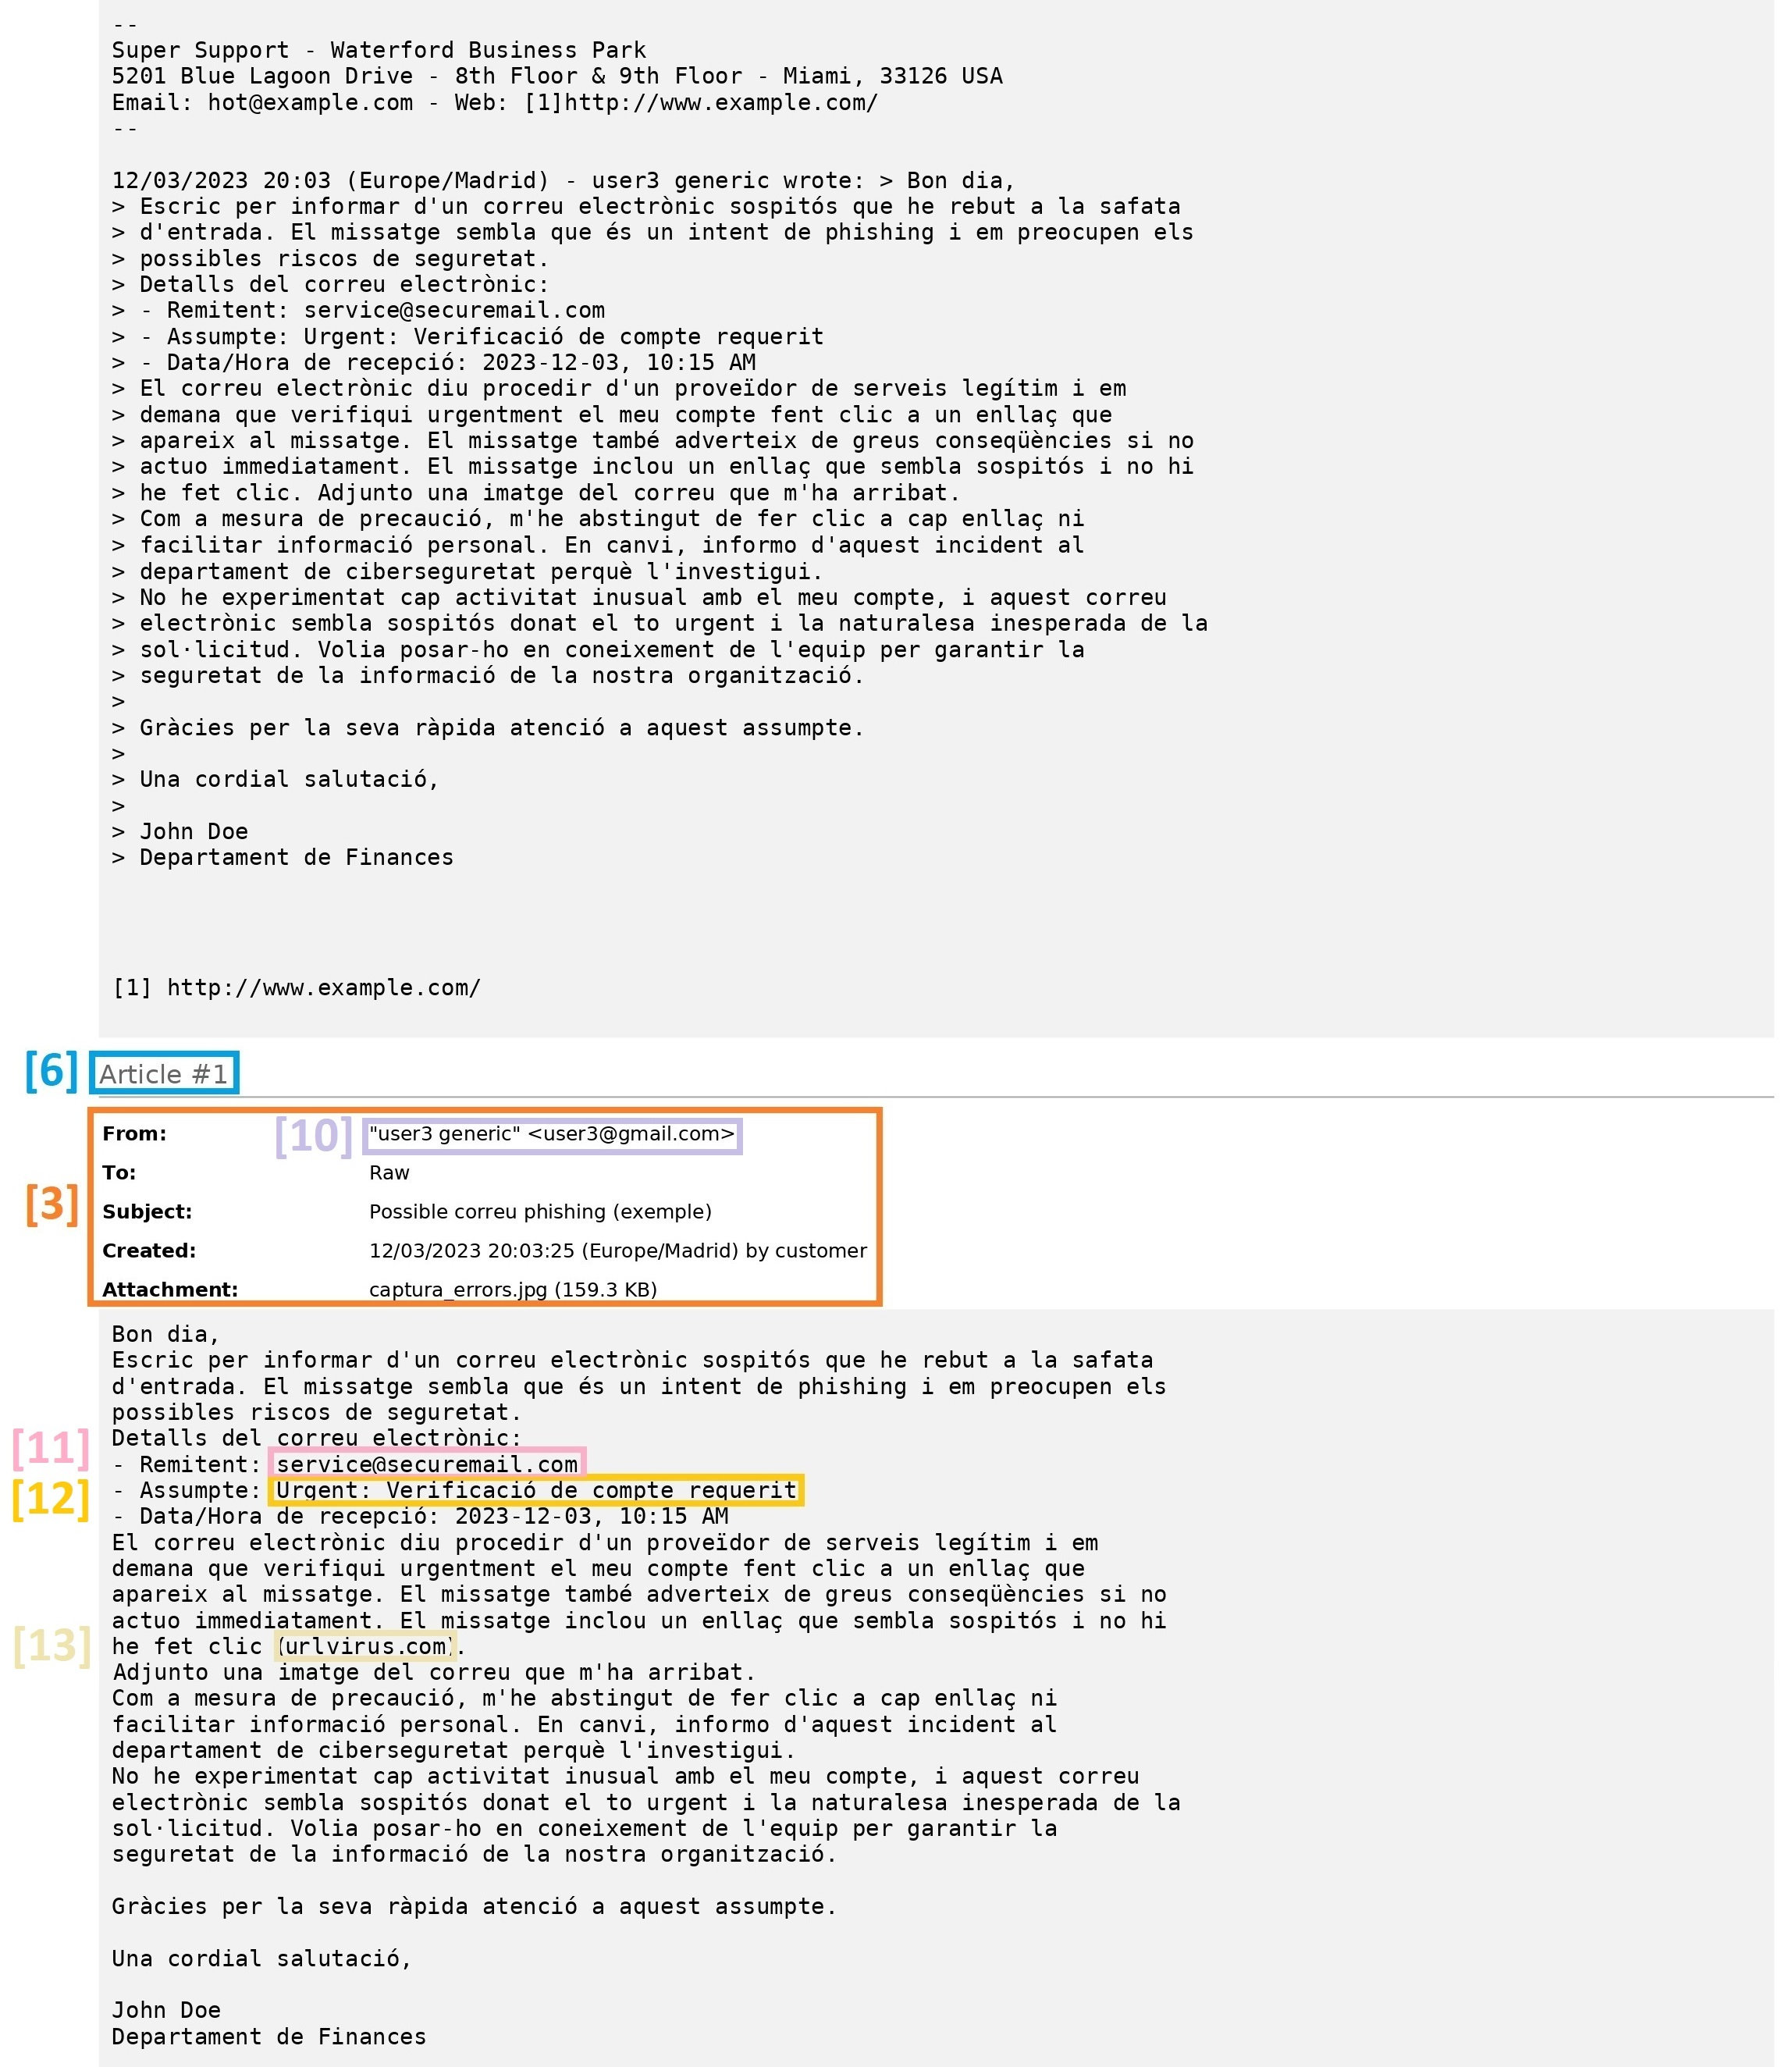
\includegraphics[width=\textwidth]{meitat-2.png}
    \caption{Segona meitat del tiquet d'exemple d'ORTS amb totes les parts indicades. \\ \textit{(Creació pròpia)}}
    \label{fig:tiquet-exemple-2}
\end{figure}

\begin{enumerate}
  \setcounter{enumi}{6}
  \item Usuaris afectats
  \item Accions de mitigació
  \item Accions de control
  \item Mail de la víctima que informa
  \item Mail de l'atacant
  \item Assumpte correu de l'incident
  \item URL de l'incident
  \item Mail de la víctima
\end{enumerate}

\subsubsection{NLP}
 El \textit{Natural Language Processing} també conegut per les seves sigles en anglès \textit{NLP}, és una branca de la intel·ligència artificial que utilitza algorismes i models per a la comprensió i generació de text.
\subsubsection{Non-Disclosure Agreement (NDA)}
\subsubsection{Phishing/programari maliciós}
\subsubsection{dataset}
